\documentclass[12pt]{report}
\usepackage[utf8]{inputenc}
\usepackage[russian]{babel}
%\usepackage[14pt]{extsizes}
\usepackage{listings}

\usepackage{graphicx}
\graphicspath{{src/}}
\DeclareGraphicsExtensions{.pdf,.png,.jpg}

% Для листинга кода:
\lstset{ %
language=c++,                 % выбор языка для подсветки (здесь это С)
basicstyle=\small\sffamily, % размер и начертание шрифта для подсветки кода
numbers=left,               % где поставить нумерацию строк (слева\справа)
numberstyle=\tiny,           % размер шрифта для номеров строк
stepnumber=1,                   % размер шага между двумя номерами строк
numbersep=5pt,                % как далеко отстоят номера строк от подсвечиваемого кода
showspaces=false,            % показывать или нет пробелы специальными отступами
showstringspaces=false,      % показывать или нет пробелы в строках
showtabs=false,             % показывать или нет табуляцию в строках
frame=single,              % рисовать рамку вокруг кода
tabsize=2,                 % размер табуляции по умолчанию равен 2 пробелам
captionpos=t,              % позиция заголовка вверху [t] или внизу [b] 
breaklines=true,           % автоматически переносить строки (да\нет)
breakatwhitespace=false, % переносить строки только если есть пробел
escapeinside={\#*}{*)}   % если нужно добавить комментарии в коде
}

% Для измененных титулов глав:
\usepackage{titlesec, blindtext, color} % подключаем нужные пакеты
\definecolor{gray75}{gray}{0.75} % определяем цвет
\newcommand{\hsp}{\hspace{20pt}} % длина линии в 20pt
% titleformat определяет стиль
\titleformat{\chapter}[hang]{\Huge\bfseries}{\thechapter\hsp\textcolor{gray75}{|}\hsp}{0pt}{\Huge\bfseries}


% plot
\usepackage{pgfplots}
\usepackage{filecontents}
\usetikzlibrary{datavisualization}
\usetikzlibrary{datavisualization.formats.functions}


\begin{document}
%\def\chaptername{} % убирает "Глава"
\begin{titlepage}
	\centering
	{\scshape\LARGE МГТУ им. Баумана \par}
	\vspace{3cm}
	{\scshape\Large Лабораторная работа №3\par}
	\vspace{0.5cm}	
	{\scshape\Large По курсу: "Анализ алгоритмов"\par}
	\vspace{1.5cm}
	{\huge\bfseries Алгоритмы сортировки\par}
	\vspace{2cm}
	\Large Работу выполнил: Гаврилов Дмитрий, ИУ7-56Б\par
	\vspace{0.5cm}
	\LargeПреподаватели:  Волкова Л.Л., Строганов Ю.В.\par

	\vfill
	\large \textit {Москва, 2019} \par
\end{titlepage}

\tableofcontents

\newpage
\chapter*{Введение}
\addcontentsline{toc}{chapter}{Введение}

На данный момент существует огромное количество вариаций сортировок.
Эти алгоритмы необходимо уметь сравнивать, чтобы выбирать наилучше подходящие в конкретном случае. 

Эти алгоримы оцениваются по:

\begin{itemize}
	\item Времени быстродействия
\end{itemize}

Целью данной лабораторной работы является изучение применений алгоритмов сортировки, обучение расчету трудоемкости алгоритмов.


\chapter{Аналитическая часть}
\section{Описание алгоритмов}
Сортировка массива — одна из самых популярных операций над массивом. Алгоритмы реализуют упорядочивание элементов в списке.
 В случае, когда элемент списка имеет несколько полей, поле, служащее критерием порядка, называется ключом сортировки
\textbf{Область применения:} 
\begin{itemize}
  	\item физика,
	\item математика,
	\item экономика,
	\item итд.
\end{itemize}

\subsection{Сортировка пузырьком}
Алгоритм проходит по массиву {n-1} раз или до тех пор, пока массив не будет полностью отсортирован. 
В каждом проходе элементы попарно сравниваются и, при необходимости, меняются местами.
При каждом проходе алгоритма по внутреннему циклу, очереднй наибольший элемент ставится на своё место в конец неотсортированного массива. 
Таким образом наибольшие элементы "всплывают" как пузырек. 

\subsection{Сортировка вставками}
На каждом шаге выбирается один из элементов неотсортированной части массива (максимальный/минимальный) 
и помещается на нужную позицию в отсортированную часть массива. 

\subsection {Быстрая сортировка}
Массив разбивается на два (возможно пустых) подмассива. Таких, что в одном подмассиве каждый элемент меньше либо равен опорному, 
и при этом не превышает любой элемент второго подмассива. Опорный элемент вычислыется в ходе процедуры разбиения. 
Подмассивы сортируются с помощью рекурсивного вызова процедуры быстрой сортировки. 
Поскольку подмассивы сортируются на месте, для их объединения не трубуются никакие действия.


\chapter{Конструкторская часть}
\section{Схемы алгоритмов}
В данном разделе будут рассмотрены схемы алгоритмов пузырьком с флагом (\ref{ris:imageSB}), сортировки вставками (\ref{ris:imageSI}), быстрой сортировки (\ref{ris:imageSQ}).

\newpage
\begin{figure}[h]
\center{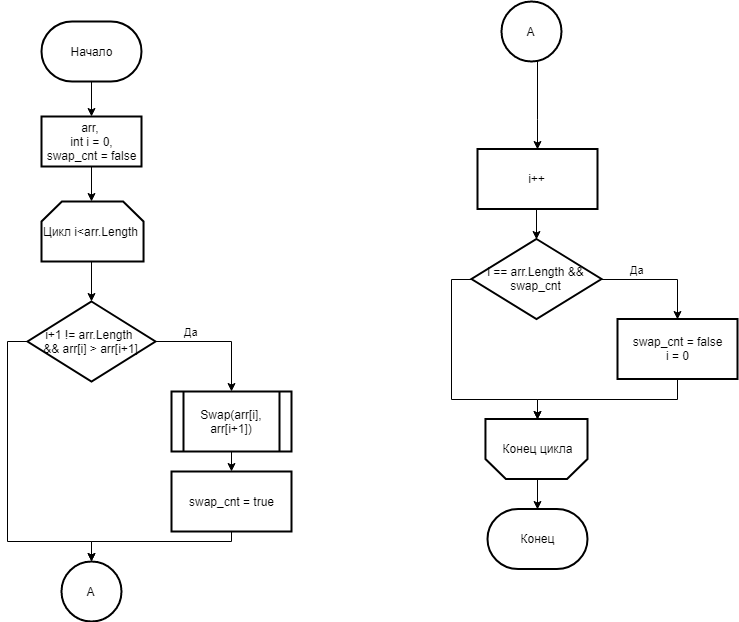
\includegraphics[height = 12cm]{Bubble}}
\caption{Схема алгоритма сортировки пузырьком с флагом}
\label{ris:imageSB}
\end{figure}

\newpage
\begin{figure}[h]
\center{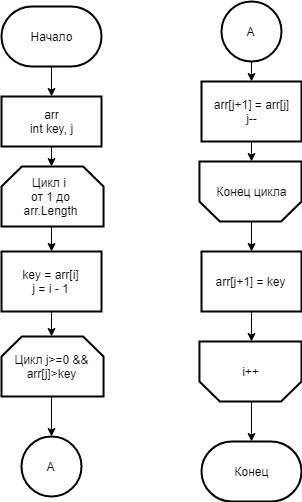
\includegraphics[height = 12cm]{Insertion}}
\caption{Схема алгоритма сортировки вставками}
\label{ris:imageSI}
\end{figure}

\newpage
\begin{figure}[h]
\center{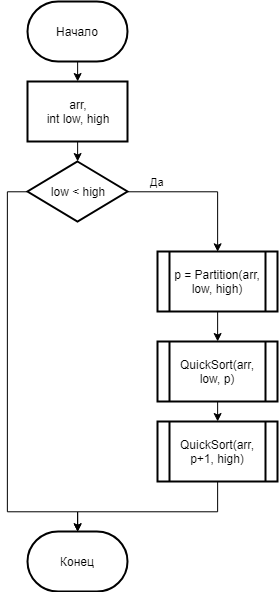
\includegraphics[scale=0.53]{Quick}}
\caption{Схема алгоритма быстрой сортировки}
\label{ris:imageSQ}
\end{figure}

\newpage
\begin{figure}[h]
\center{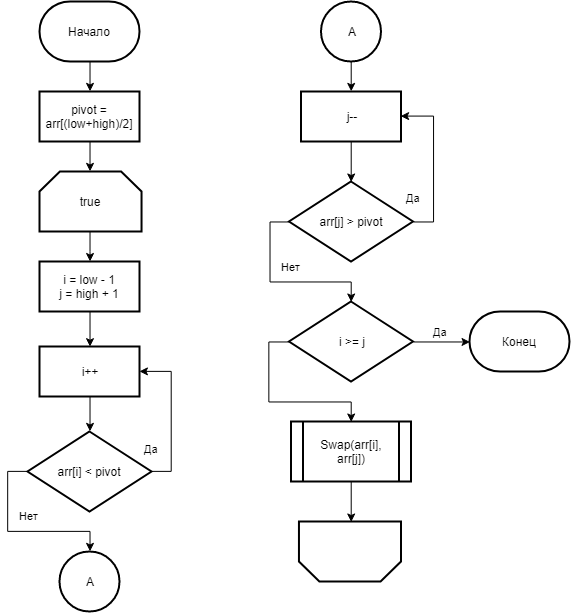
\includegraphics[height = 12cm]{Partition}}
\caption{Схема функции partition}
\label{ris:imageSP}
\end{figure}


\section{Трудоемкость алгоритмов}
Введем модель трудоемкости для оценки алгоритмов:
\begin{enumerate}
  	\item  базовые операции стоимостью 1 — +, -, *, /, =, ==, <=, >=, !=, +=, [], получение полей класса
	\item оценка трудоемкости цикла: Fц = a + N*(a + Fтела), где a - условие цикла
	\item стоимость условного перехода возьмем за 0, стоимость вычисления условия остаётся.
\end{enumerate}

Далее будет приведены оценки трудоемкости алгоритмов. Построчная оценка трудоемкости сортировки пузырькм с флагом (Табл. 2.1).

\subsection{Сортировка пузырьком с флагом}
\begin{center}
Табл. 2.1 Построчная оценка веса
	\begin{tabular}{|l c|} 
 	\hline
	Код & Вес \\ [0.5ex] 
 	\hline\hline
 	 int i = 0; & 1\\
 	\hline
	bool swapcnt = false; & 1\\
	\hline
	while (i < arr.Length) & 2\\
	\hline
	\{ & 0\\
	\hline
	if(i + 1 != arr.Length \&\& arr[i] > arr[i + 1]) & 7\\
	\hline
	\{ & 0\\
	\hline
	Swap(ref arr[i], ref arr[i + 1]); & 2+3\\
	\hline
	swapcnt = true; & 1\\
	\hline
	\} & 0\\
	\hline
	i++; & 1\\
	\hline
	if (i == arr.Length \&\& swapcnt) & 3\\
	\hline
	\{ & 0\\
	\hline
	swapcnt = false; & 1\\
	\hline
	i = 0; & 1\\
	\hline
	\} & 0\\
	\hline
	\} & 0\\
	\hline
	\end{tabular}
\end{center}

 
\textbf{Лучший случай:} Массив отсортирован; не произошло ни одного обмена за 1 проход -> выходим из цикла \newline
Трудоемкость:  $1 + 1 + n* (2 + 7 + 1 + 3 ) + 2 = 13n + 4 = O(n)$

\textbf{Худший случай:}  Массив отсортирован в обратном порядке; в каждом случае происходил обмен\newline
Трудоемкость: $1 + 1 +  n*(n* (7 + 5 + 1  + 3)  + 1 + 1) + 2 =  n*(16n + 2) + 4 = 16n^2 + 2n + 4 = O(n^2)$


\subsection{Сортировка вставками}
\hspace*{5mm}
\textbf{Лучший случай:} отсортированный массив. При этом все внутренние циклы состоят всего из одной итерации.\newline
Трудоемкость: $T(n) = 3n + ((2 + 2 + 4 + 2 ) * (n - 1))  =  3n + 10(n-1) = 13n - 10 = O(n)$

\textbf{Худший случай:} массив отсортирован в обратном нужному порядке. Каждый новый элемент сравнивается со всеми в отсортированной последовательности.
Все внутренние циклы будут состоять из j итераций. \newline
Трудоемкость: $T(n) = 3n + (2 + 2)(n-1) + 4 \left({\frac {n(n+1)}{2}}-1\right)+5{\frac {n(n-1)}{2}}+3(n-1) = 3n + 4n - 4 + 2n^2
+ 2n - 4 + 2.5n^2 - 2.5n + 3n - 3 = 4.5n^2 + 9.5n - 11 = O(n^{2})$

\subsection{Быстрая сортировка}
\hspace*{5mm}
\textbf{Лучший случай:} сбалансированное дерево вызовов \(O(n*log(n))\)  
В наиболее благоприятном случае процедура PARTITION приводит к двум подзадачам, размер каждой из которых не превышает $\frac{n}{2}$, поскольку размер одной из них равен $\frac{n}{2}$ , а второй$\frac{n}{2} - 1$. В такой ситуации быстрая сортировка работает намного производительнее, и время ее работы описывается следующим рекуррентным соотношением: $T(n) = 2T(\frac{n}{2}) + O(n)$,где мы не обращаем внимания на неточность, связанную с игнорированием функций “пол” и “потолок”, и вычитанием 1. Это рекуррентное соотношение имеет решение ; $T(n) =O(nlgn)$. При сбалансированности двух частей разбиения на каждом уровне рекурсии мы получаем асимптотически более быстрый алгоритм.

Фактически любое разбиение, характеризующееся конечной константой пропорциональности, приводит к образованию дерева рекурсии высотой $O(lgn)$ со стоимостью каждого уровня, равной $O(n)$. Следовательно, прилюбой постоянной пропорции разбиения полное время работы быстрой сортировки составляет $O(nlgn)$.

\textbf{Худший случай:} несбалансированное дерево $O(n^2)$
Поскольку рекурсивный вызов процедуры разбиения, на вход которой подается массив размером 0, приводит к немедленному возврату из этой процедуры без выполнения каких-ли-бо операций, $T(0) = O(1)$. Таким образом, рекуррентное соотношение, описывающее время работы процедуры в указанном случае, записывается следующим образом: 
$T(n) =T(n-1) +T(0) + O(n) =T(n-1) + O(n)$. Интуитивно понятно, что при суммировании промежутков времени, затрачиваемых на каждый уровень рекурсии, получается арифметическая прогрессия, что приводит к результату $O(n^2)$.

\section{Вывод}
Сортировка пузырьком: лучший - $O(n)$, худший - $O(n^2)$ \newline
Сортировка вставками: лучший - $O(n)$, худший - $O(n^2)$ \newline
Быстрая сортировка: лучший - $O(nlgn)$, худший - $O(n^2)$ \newline

При этом сортировка вставками быстрее пузырька с флагом в худшем случае т.к. имеет меньший коэффициент. Вставки $4.5n^2$, пузырек $16n^2$.


\chapter{Технологическая часть}
\section{Выбор ЯП}
В качестве языка программирования был выбран Java, а средой разработки Intellij IDEA.
Время работы алгоритмов было замерено с помощью класса Instant.

\section{Описание структуры ПО}

\section{Сведения о модулях программы}
Программа состоит из:
\begin{itemize}
	\item Main.java - главный файл программы, в котором располагается точка входа в программу и функция замера времени.
	\item SortUtils.java - файл класса sorting, в котором находятся алгоримы сортировки
	\item RandomArrayFactory.java - файл-фабрика для генерации различных массивов
\end{itemize}

\section{Листинг кода}
\begin{lstlisting}[label=bubble,caption=Алгоритм сортировки пузырьком]
public static void bubbleSort(int[] array) {  
    boolean sorted = false;
    int temp;
    while(!sorted) {
        sorted = true;
        for (int i = 0; i < array.length - 1; i++) {
            if (array[i] > array[i+1]) {
                temp = array[i];
                array[i] = array[i+1];
                array[i+1] = temp;
                sorted = false;
            }
        }
    }
}
\end{lstlisting}
\newpage
\begin{lstlisting}[label=insertion,caption=Алгоритм сортировки вставками]
public static void insertionSort(int[] array) {  
    for (int i = 1; i < array.length; i++) {
        int current = array[i];
        int j = i - 1;
        while(j >= 0 && current < array[j]) {
            array[j+1] = array[j];
            j--;
        }
        
        array[j+1] = current;
    }
}
\end{lstlisting}

\begin{lstlisting}[label=quick,caption=Алгоритм быстрой сортировки]
public static void quickSort(int[] array, int begin, int end) {  
    if (end <= begin) return;
    int pivot = partition(array, begin, end);
    quickSort(array, begin, pivot-1);
    quickSort(array, pivot+1, end);
}
\end{lstlisting}

\begin{lstlisting}[label=pivot,caption=Алгоритм поиска опорного элемента]
public static int partition(int[] array, int begin, int end) {  
    int pivot = end;

    int counter = begin;
    for (int i = begin; i < end; i++) {
        if (array[i] < array[pivot]) {
            int temp = array[counter];
            array[counter] = array[i];
            array[i] = temp;
            counter++;
        }
    }
    int temp = array[pivot];
    array[pivot] = array[counter];
    array[counter] = temp;

    return counter;
}
\end{lstlisting}


\section{Вывод}
В данном разделе были представлены реализации алгоритмов сортировки пузырьком, вставками и быстрой сортировки.

\chapter{Исследовательская часть}
Был проведен замер времени работы каждого из алгоритмов.

\section{Примеры работы программы}
\begin{figure}[h]
\center{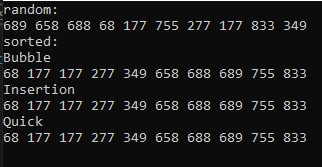
\includegraphics[scale=1]{Test1}} 
\caption{Сортировка массива, заполненного случайными числами}
\label{ris:image}
\end{figure}
\newpage
\begin{figure}[h]
\center{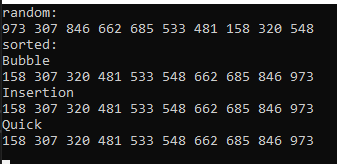
\includegraphics[scale=1]{Test2}} 
\caption{Сортировка массива, заполненного случайными числами}
\label{ris:image}
\end{figure}

\begin{figure}[h]
\center{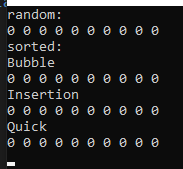
\includegraphics[scale=1]{Same}} 
\caption{Сортировка массива, заполненного одинаковыми числами}
\label{ris:image}
\end{figure}
\newpage
\begin{figure}[h]
\center{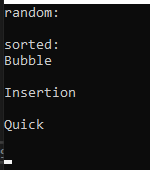
\includegraphics[scale=1]{Empty}} 
\caption{Сортировка пустого массива}
\label{ris:image}
\end{figure}

\section{Эксперимент}
В рамках данного эксперимента было произведено сравнение времени выполнения трех алгоритмов в лучшем/худшем/случайном
случае заполения массива. При длине массивов от 100 до 1000 элементов с шагом 100. На предоставленных ниже графиках Рис. 4.1, Рис. 4.2, Рис. 4.3
по оси l идет длина массива, а по оси t - время сортировки в милисекундах.

\begin{tikzpicture}
\begin{axis}[
    	axis lines = left,
    	xlabel = Размер массива,
    	ylabel = Время (мс),
	legend pos=north west,
	ymajorgrids=true
]
\addplot[color=red, mark=square] table[x index=0, y index= 1] {BubbleAsc.txt}; 
\addplot[color=blue, mark=square] table[x index=0, y index= 1] {InsertionAsc.txt}; 
\addplot[color=green, mark=square] table[x index=0, y index= 1] {QuickAsc.txt}; 

\addlegendentry{BubbleSort}
\addlegendentry{InsertionSort}
\addlegendentry{QuickSort}
\end{axis}
\end{tikzpicture}
\begin{center}
Pис. 4.1: Сравнение времени для отсортированного массива
\end{center}


\begin{tikzpicture}
\begin{axis}[
    	axis lines = left,
    	xlabel = Размер массива,
    	ylabel = Время (мс),
	legend pos=north west,
	ymajorgrids=true
]
\addplot[color=red, mark=square] table[x index=0, y index= 1] {BubbleDec.txt}; 
\addplot[color=blue, mark=square] table[x index=0, y index= 1] {InsertionDec.txt}; 
\addplot[color=green, mark=square] table[x index=0, y index= 1] {QuickSame.txt}; 

\addlegendentry{BubbleSort}
\addlegendentry{InsertionSort}
\addlegendentry{QuickSort}
\end{axis}
\end{tikzpicture}
\begin{center}
Pис. 4.2: Сравнение времени для отсортированного массива в обратном порядке
\end{center}


\begin{tikzpicture}
\begin{axis}[
    	axis lines = left,
    	xlabel = Размер массива,
    	ylabel = Время (мс),
	legend pos=north west,
	ymajorgrids=true
]
\addplot[color=red, mark=square] table[x index=0, y index= 1] {BubbleRnd.txt}; 
\addplot[color=blue, mark=square] table[x index=0, y index= 1] {InsertionRnd.txt}; 
\addplot[color=green, mark=square] table[x index=0, y index= 1] {QuickRnd.txt}; 

\addlegendentry{BubbleSort}
\addlegendentry{InsertionSort}
\addlegendentry{QuickSort}
\end{axis}
\end{tikzpicture}
\begin{center}
Pис. 4.3: Сравнение времени при случайном заполнении массива
\end{center}

\section{Вывод}
По результатам тестирования выявлено, что все рассматриваемые алгоритмы реализованы правильно. Самым быстрым алгоритмом, при использовании случайного заполнения, оказался алгоритм быстрой сортировки, а самым медленным — алгоритм сортировки пузырьком.

\chapter*{Заключение}
\addcontentsline{toc}{chapter}{Заключение}
В ходе работы были изучены алгоритмы сортировки массива: пузырьком с флагом, вставки, быстрая сортировка. Выполнено сравнение всех рассматриваемых алгоритмов. В ходе исследования был найден оптимальный алгоритм. Изучены зависимости выполнения алгоритмов от длины массива. Также реализован программный код продукта.


\chapter*{Список литературы}
\addcontentsline{toc}{chapter}{Список литературы}
\begin{enumerate}
	\item Кормен Т. Алгоритмы: построение и анализ [Текст] / Кормен Т. - Вильямс, 2014. - 198 с. - 219 с.
\end{enumerate}

\end{document}